\subsection{Realizing LBM Models Computationally}
Because of the immensely simple implementation of no-slip boundary conditions for even the most complex geometry, the lattice-Boltzmann method was immediately seen as a powerful option of fluid modeling in porous networks. Chen \& Doolen review many of the major accomplishments of implementing LBM models which verified Darcy's Law, the Cozeny-Karman equation, and Brinkmann equation, among other efforts.\cite{Chen1998a} Pan\etal~evaluated the single-relaxation time BGK operator against models with multiple relaxation times as well as models with different implementationsi of fluid-solid interface boundary conditions -- among which was the bounce-back scheme we use here.\cite{Pan2006}

Here we will go through the practical application of the LBM approach as it will be used  to simulate the conjugate heat transfer of the helium purge gas through ceramic pebble beds. To summarize the method, there are two main objects required to define the structure of a lattice-Boltzmann model: a collision operator, $\Omega_i$, and the constants which define the scaffolding of the lattice.

The computational domain of the fluid is discretized into a Cartesian grid with regularized spacing, $\delta_x$, in every dimension. At each node are density functions, $f_i(\vec{x},t)$, which represent the density at that node (found at $\vec{x}$), traveling in the direction of $\vec{c}_i$ at a moment in time, $t$. The density distribution function evolves according to Eq.~\ref{eq:lbm-evolution}. It is helpful to look at the equation compartmentalized in the same manner it is handled computationally, thus we see the streaming and collision parts,
\begin{align}
	\underbrace{f_i(\vec{x}+\vec{c}_i, t + 1)  = f_i(\vec{x},t)}_\text{streaming}  + \underbrace{\Omega_i(\vec{x},t)}_\text{collision}
\end{align}

Conceptually the two steps of the evolution can be thought of as two distinct operations. First, the collision operator is calculated based only on each nodes local information. Using the BGK approximation, given in Eq.~\ref{eq:bgk-operator}, the collision is calculated as
\begin{align}
	\Omega_i = -\frac{1}{\tau}\left[f_i(\vec{x},t) - f_i^\eq(\vec{x},t)\right]
\end{align}

Post-collision, in the streaming step, the information is passed from every node to its neighbors along the lattice directions shown in Fig.~\ref{fig:d3q19-lattice}. While the collision operation is exactly local, the streaming operation involves only nearest neighbors. After the streaming step, the nodes that lie along the boundary have the bounce-back scheme applied wherein distributions arriving at the boundary are reflected back to their incident directions. The bounce-back calculation enforces no-slip at the walls.

Splitting the evolution of the distribution function into the two steps of collision and streaming, in addition to being a conceptual aid, is a natural partition of computational steps. In practice the algorithm proceeds as follows,\cite{Viggen2009}
\begin{enumerate}
	\item{using macroscopic properties of density and fluid velocity, the equilibrium distribution function is calculated at every node following Eq.~\ref{eq:equilib-dist-function},}
	\item{the BGK collision operator is calculated according to Eq.~\ref{eq:bgk-operator} to find the post-collision distribution of every node,}
	\item{information from each node streaming to neighboring nodes based on the evolution equation of Eq.~\ref{eq:lbm-evolution},}
	\item{updated macroscopic properties are found from the new distribution functions according to Eq.~\ref{eq:lbm2physical}.}
\end{enumerate}

It is worth stressing again that the lattice-Boltzmann collision calculations are completely local, with the streaming step requiring only nearest inter-node communication for updating distribution functions which lends the method to extremely efficient parallelization. We now need a means of translating physical properties into lattice units. Then we can incorporate our pebble bed into the LBM computational space before LBM simulations of helium-pebble conjugate heat transfer can be performed.





\subsection{Physical to Lattice Units}\label{sec:physical-to-lattice}
In LBM one typically works with lattice variables -- differing from their physical counterparts simply through normalization. This is akin to achieving dynamic similarity in fluid mechanics experiments with matching geometry and Reynolds numbers. I therefore will discuss the nondimensional form of governing equations and then translate the nondimensional values into lattice variables. We then see how tuning of some lattice variables will allow a sufficiently refined grid while still representing the physical system we are attempting to model. The notation of working with physical, nondimensional, and lattice variables can quickly become cumbersome. The convention I will adhere to is to use $\hat{\psi}$ for physical variables, $\psi^*$, or nondimensional variables, and simply $\psi$ for lattice variables.

Thus the Navier-Stokes equations, in physical units, for an incompressible fluid are
\begin{equation}
	\hat{\nabla}\cdot\hat{\vec{u}} = 0
\end{equation}
and
\begin{equation}
	\frac{\partial \hat{\vec{u}}}{\partial \hat{t}} + (\hat{\vec{u}}\cdot\hat{\nabla})\hat{\vec{u}} = -\frac{1}{\hat{\rho}_0}\hat{\nabla}\hat{p} + \hat{\nu}\hat{\nabla}^2\hat{\vec{u}}
\end{equation}

I nondimensionalize the length scale based on the average diameter of pebble in our system, the velocity by the superficial velocity of our inlet, and pressure and time on derived forms of these two variables,
\begin{subequations}
\begin{align}
	x^* &= \frac{\hat{x}}{\hat{d}_p} \\
	\vec{u}^* &= \frac{\hat{\vec{u}}}{\hat{\vec{u}}_i} \\
	p^* &= \frac{\hat{p}}{\hat{\rho}_0\hat{\vec{u}}_i^2}\\
	t^* &= \frac{\hat{t}}{\frac{\hat{d}_p}{\hat{\vec{u}}_i}}
\end{align}
\end{subequations}

Thus the nondimensional form of Navier-Stokes is the familiar,
\begin{subequations}\label{eq:non-dim-ns}
\begin{align}
	\nabla^* \cdot \vec{u}^* &= 0 \\
	\frac{\partial \vec{u}^*}{\partial t^*} + (\vec{u}^*\cdot\nabla^*)\vec{u}^* &= -\nabla^*p^* + \frac{1}{\Re}\nabla^{*2}\vec{u}^*
\end{align}
\end{subequations}

Note, too, that the physical limits of our system are describable in terms of the nondimensional units. In other words, if our system is $\hat{X}$ meters wide, the nondimensional width is $X^*=\frac{\hat{X}}{\hat{d}_p}$.  

% The last thing we need before converting the variables of Eq.~\ref{eq:non-dim-ns} into lattice units are the lattice spacing and lattice time step, $\delta_x$ and $\delta_t$. We will define the lattice spacing based on the resolution of our pebble diameter, as described above.

The manner of description I will follow next will match the method in which the values are actually programmed in my DEM-to-LBM script. I begin by defining the pebble diameter, limits, and resolution ($\text{res}$); the script returns $\delta_x$, $N_x$, $N_y$, and $N_z$ where the $N$ values represent the total number of nodes in a given direction. The values are calculated as,
\begin{subequations}
\begin{align}
	\delta_x = \delta_y = \delta_z & = \frac{1}{\text{res}} \\
	N_x & = \text{res}\cdot X^* \\
	N_y & = \text{res}\cdot Y^* \\
	N_z & = \text{res}\cdot Z^*
\end{align}
\end{subequations}

Recalling that the description of the lattice evolution equations requires a relaxation time that is based on the lattice viscosity, the property is defined on the lattice as,
\begin{equation}
	\nu = \frac{\delta_t}{\delta_x^2}\frac{1}{\Re}
\end{equation}
from which, the relaxation time for our single-relaxation-time, D3Q19 lattice is calculated from Eq.~\ref{eq:lbm-viscosity-relaxation-time} as,
\begin{equation}
	\tau_{ns} = \frac{\nu}{c_s^2} + \frac{1}{2}
\end{equation}
where the subscript $_{ns}$ denotes the relaxation time is specific for the fluid flow as described by the Navier-Stokes equations and the lattice speed of sound is $c_s^2 = \frac{1}{3}$.

To specify the velocity boundary condition (and similarly to convert our lattice velocity results back into physical values), we must have a translator between nondimensional and lattice velocities,
\begin{equation}\label{eq:lbm-u}
	\vec{u} = \frac{\delta_t}{\delta_x}\vec{u}^*
\end{equation}

Translating from physical to lattice units is done via,
\begin{equation}
	u = \frac{\delta_t}{\delta_x}\frac{\hat{\vec{u}}}{\hat{\vec{u}}_i}
\end{equation}
and the translation is used, for instance, when defining the boundary velocity in the lattice based on the predefined physical velocity.

The only lattice parameter not defined at this point is the lattice time step, $\delta_t$. In lattice-Boltzmann, $\delta_t$ and $\delta_x$ are linked via the incompressibility constraint in the lattice. At the same time, from Eq.~\ref{eq:lbm-u}, the lattice velocity is directly related to the lattice time step size; and the magnitude of $\vec{u}$ may not be larger than the speed of sound on the lattice, $c_s$. The time step is further constrained when enforcing incompressibility of our fluid. The LB model is a quasi-compressible fluid solver which permits slight compressible regimes to enter the system to solve the pressure equation of the fluid. Compressibility effects will impact the numerical accuracy and should therefore be minimized. As these effects scale like the square Mach-number, $\Ma^2$, compressibility effects can be minimized by enforcing a small Mach number. In LBM, the lattice Mach number is simply,
\begin{equation}
 	\Ma = \frac{|\vec{u}_0|}{c_s}
\end{equation}
where $|\vec{u}_0| = \frac{\delta_t}{\delta_x}$. Thus to say the compressibility error scales like $\epsilon \sim \Ma^2$ is to say it scales like $\epsilon \sim \frac{\delta_t^2}{\delta_x^2}$. The compressibility error need not be smaller than the numerical error of the LBM method itself. As LB is second-order accurate\cite{succi2001lattice}, $\epsilon \sim \delta_x^2$, we can then determine the time step size relative to lattice spacing for which the two errors will be comparable in size,
\begin{align*}
	\frac{\delta_t^2}{\delta_x^2} &\sim \delta_x^2\\
	\rightarrow \delta_t &\sim \delta_x^2
\end{align*}

Also, because the lattice spacing is directly dependent on our chosen resolution, the requirement on time step is alternatively written as
\begin{equation}
	\delta_t \sim \frac{1}{\text{res}^2}
\end{equation}
which shows, similar to standard CFD solvers, the time step requirement shrinks rapidly as we attempt to more finely represent the pebbles with more and more nodes. Thus care must be taken to balance the resolution with the time step requirements.

In the LBM model, we only treat the energy as a passive scalar transported by the fluid motion (\textit{i.e.} we do not make the Boussinesq approximation to couple the fluid energy to momentum). The energy equation for the fluid in physical units is,
\begin{equation}
	\frac{\partial \hat{T}_f}{\partial \hat{t}} + \hat{\nabla}\cdot(\hat{\vec{u}}\,\hat{T}_f) = -\hat{\alpha}_f\hat{\nabla}^2\hat{T}_f
\end{equation}

The temperature will be nondimensionalized based on a characteristic temperature of volumetric heating,
\begin{equation}
	T^* = \frac{\hat{T}}{\hat{q}''' \hat{d}_p^2/\hat{k}_s}
\end{equation}
and the time and length scales are nondimensionalized as in the Navier-Stokes equations. Thus the nondimensional energy equation is
\begin{equation}\label{eq:non-dim-energy}
	\frac{\partial T^*_f}{\partial t^*} + \nabla^*(u^*T^*_f) = -\frac{1}{\Pe_f} \nabla^{*2}T^*_f
\end{equation}
where $\Pe$ is the Peclet number ($\Pe = \Re\cdot \Pr$). The Peclet number for the fluid and solid will be unique, hence we must distinguish them with a fluid/solid subscript.

To discretize the dimensionless energy system into the lattice, we recognize the similarities between Eq.~\ref{eq:non-dim-ns} and Eq.~\ref{eq:non-dim-energy} to directly write the lattice thermal diffusivity of the fluid as
\begin{equation}
	\alpha_f = \frac{\delta_t}{\delta_x^2}\frac{1}{\Pe_f}
\end{equation}

For the solid, the energy equation in dimensional units is
\begin{equation}
	\frac{\partial \hat{T}_s}{\partial \hat{t}} = -\hat{\alpha}_s\hat{\nabla}^2\hat{T}_s + \frac{\hat{q}'''}{\hat{\rho}_s\hat{C}_{ps}}
\end{equation}

which similarly nondimensionalizes to,
\begin{equation}\label{eq:non-dim-energy-solid}
	\frac{\partial T^*_s}{\partial t^*} = -\frac{1}{\Pe_s} \nabla^{*2}T^*_s + \frac{1}{\Pe_s}
\end{equation}
where the solid Peclet number is defined in terms of the fluid velocity and viscosity. For this Peclet number, the Reynolds number is $\Re = \frac{\hat{u}_i \hat{d}_p}{\hat{\nu}_f}$ and the Prandtl number is an awkward $\Pr = \frac{\hat{\nu}_f}{\hat{\alpha}_s}$. 

We can now directly write the lattice thermal diffusivity of the solid as
\begin{equation}
	\alpha_s = \frac{\delta_t}{\delta_x^2}\frac{1}{\Pe_s}
\end{equation}

On the thermal lattice, we need only use a D3Q7 to satisfy isotropy, for which the lattice speed of sound is only $c_s^2 = \frac{1}{2}$ (I will refer to it as $c_{s,ad}$ to distinguish). On this lattice, we are solving the energy equation for both the fluid and solid, so each material has a unique relaxation time. I will refer to them as the advection-diffusion (ad) and conjugate (cj) relaxation times, for short. They are,
\begin{subequations}
\begin{align}
	\tau_{ad} &= \frac{\alpha_f}{c_{s,ad}^2} + \frac{1}{2} \\
	\tau_{cj} &= \frac{\alpha_s}{c_{s,ad}^2} + \frac{1}{2}
\end{align}
\end{subequations}
and the size of lattice spacing and time steps are equal to those of the Navier-Stokes lattice.

To summarize the unit conversion process described above, our lattice needs to be defined in terms of lattice spacing and time step. These values can be determined from considerations of fidelity and error minimization. The physics of the system are encompassed in the relaxation time -- values which can be determined completely from lattice spacing and nondimensional values of the Reynolds number and Peclet number. Physical boundary conditions of velocity and temperature can be enforced in the lattice with translations into lattice variables as given above. %Perhaps not obvious from this discussion is that we could be free to model a fictitious fluid that allows for high numeric accuracy and stability provided that the nondimensional variables be translatable to proper physical ones.




\subsection{Mapping DEM Pebbles onto LBM Nodes}\label{sec:dem2lbm-mapping}

Unlike the dynamic coupling between DEM and the volume-averaged CFD where information passed back and forth between fluid and particle, in the LBM construction I am simply translating a static packing structure from DEM into the LBM framework. The lattices of the LBGK solver use equally spaced nodes that discretize our volume into regular spacing. The pebble data from DEM is mapped onto the LBM nodes with a script via knowledge of the centroid and radius of each pebble. To demonstrate, in Fig.~\ref{fig:dem-2-lbm-example1}, we see a two-dimensional slice of a pebble projected onto a section of an LBM lattice. If the distance from a node to the centroid is less than the radius of the pebble, the node is assigned as a solid. All other nodes are assigned as fluids.

\begin{figure}[ht]
	\centering
	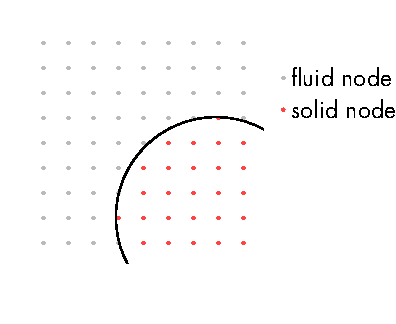
\includegraphics[width=\singleimagewidth]{chapters/figures/lbm/dem-to-lbm-mapping.pdf}
	\caption{An example of the mapping process from DEM to LBM structures. Nodes are assigned as fluid or solid based on relative location of pebble centroid and radius. Here we have a resolution of 9 (\textit{i.e.} 9 nodes per pebble diameter).}\label{fig:dem-2-lbm-example1}
\end{figure}
\begin{figure}[ht]
	\centering
	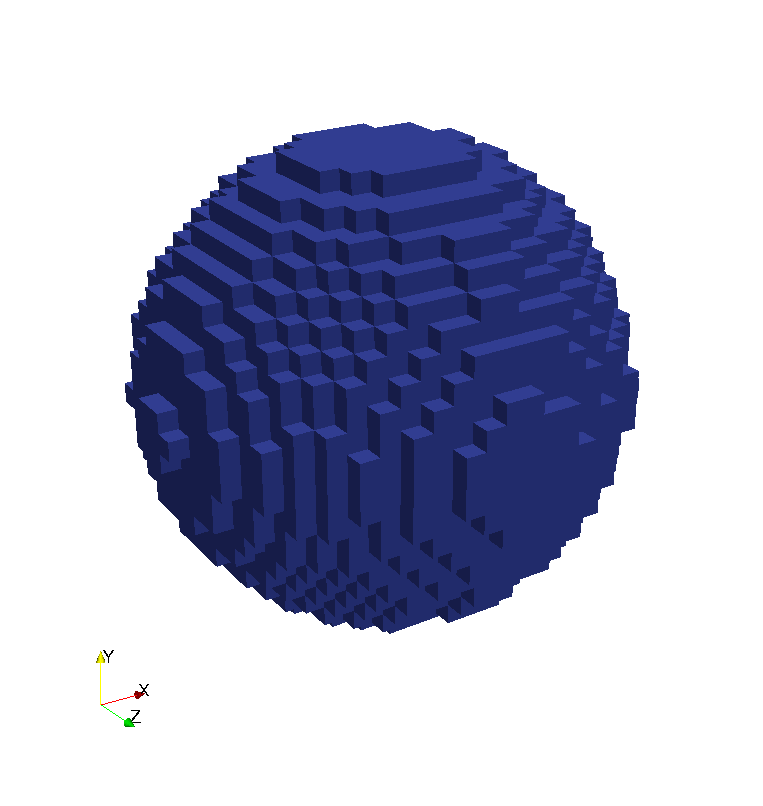
\includegraphics[width=\doubleimagewidth]{chapters/figures/lbm/lbm-pebble-res25.png}
	\caption{A three-dimensional DEM pebble as imported into the LBM lattice with a resolution of 25.}\label{fig:dem-2-lbm-example2}
\end{figure}
\begin{figure}[ht]
	\centering
	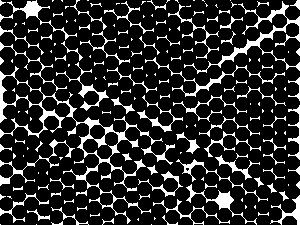
\includegraphics[width=\doubleimagewidth]{chapters/figures/lbm/crossSection0024.jpg}
	\caption{A two-dimensional slice of a DEM pebble bed as imported into the LBM lattice with a resolution of 25.}\label{fig:dem-2-lbm-example3}
\end{figure}
\begin{figure}[ht]
	\centering
	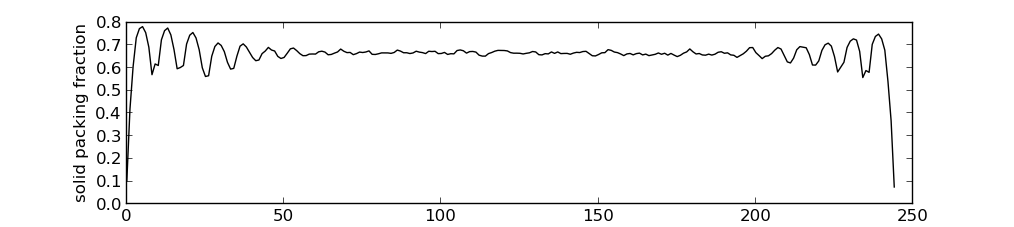
\includegraphics[width=\textwidth]{chapters/figures/lbm/palabos_packing_fraction}
	\caption{The digital packing fraction was measured at all slices through the height of the pebble bed. When the average value equaled the expected value, the mapping from DEM to LBM was considered consistent.}\label{fig:dem-2-lbm-packing-fraction}
\end{figure}

In the example of Fig.~\ref{fig:dem-2-lbm-example1}, the resolution is only 9. Thus 9 nodes are needed to span the diameter of a single pebble and the lattice spacing is $\delta_x = 1/9$. In the second example shown in Fig.~\ref{fig:dem-2-lbm-example2}, we see a pebble in three dimensions that has been mapped onto the LBM nodes with a resolution of 25 (thus $\delta_x = 1/25$). The trade-off between a small lattice spacing is in the ability to resolve the spherical surface of the pebble, stability, and even the ability to resolve a proper packing fraction in the pebble bed. 

Shown in Fig.~\ref{fig:dem-2-lbm-example3} is a single slice of a pebble bed with a resolution of 25 as it is mapped into LBM. Here, black pixels represent solid and white pixels are fluid. Because we are representing the surfaces of curved objects with straight lines, at the point of contact between pebbles, the mapping from DEM to LBM would occasionally over-predict the overlap between pebbles. This was measured numerically by comparing the number of white pixels to black pixels in each slice -- the digital equivalent of a packing fraction,
\begin{equation}
	\phi_{d,j} = \frac{N_\text{black}}{N_\text{white}}
\end{equation}

The total digital packing fraction of the ensemble, as mapped into LBM, is simply
\begin{equation}
	\phi_d = \frac{1}{J}\sum_j^J\phi_{d,j}
\end{equation}

where there are $J$ total slices. For example, we see in Fig.~\ref{fig:dem-2-lbm-packing-fraction} a plot of the digital packing fraction moving through the pebble bed. The digital mapping of DEM onto LBM was tweaked with a radius magnification parameter until the digital packing fraction matched the calculated packing fraction from DEM. When the error between digital and continuous packing fractions was small, as calculated by
\begin{equation}
	\Phi_{err} = \frac{|\phi_d - \phi|}{\phi} < 10^{-4}
\end{equation}
I considered the mapping from DEM to LBM to be consistent.
\FloatBarrier